\documentclass[a4paper,12pt]{article} 


\usepackage[T2A]{fontenc}			
\usepackage[utf8]{inputenc}			
\usepackage[english,russian]{babel}	

\usepackage{graphicx, scalerel}    
\usepackage{wrapfig}               
\usepackage[14pt]{extsizes}        
\usepackage[warn]{mathtext}       
\usepackage{indentfirst}      
\usepackage[margin = 25mm]{geometry}
\usepackage[table,xcdraw]{xcolor} 
\usepackage{amsmath,amsfonts,amssymb,amsthm,mathtools}
\usepackage{wasysym}                
\usepackage{upgreek}                
\usepackage{caption}
\usepackage{multirow}
\captionsetup{labelsep=period}
\usepackage[font=small,labelfont=bf]{caption}
\usepackage{gensymb}
\usepackage{icomma}

\usepackage[unicode, pdftex]{hyperref}
\usepackage{tikz}
\usetikzlibrary{positioning}
\usepackage{fancyhdr}
\pagestyle{fancy}
\setlength\fboxsep{3pt} % Отступ рамки \fbox{} от рисунка
\setlength\fboxrule{1pt} % Толщина линий рамки \fbox{}
\usepackage{tocloft}
\newcommand{\tocsection}[1]{\section*{#1} \addcontentsline{toc}{section}{#1}}
\newcommand{\tocsubsection}[1]{\subsection*{#1} \addcontentsline{toc}{subsection}{#1}}
\renewcommand{\cftsecleader}{\cftdotfill{\cftdotsep}}

\begin{document}
	\newcommand{\HRule}{\rule{\linewidth}{0.7mm}} % Defines a new command for the horizontal lines, change thickness here

\begin{center}
	\large\textbf{Московский Физико-Технический Институт}\\
	\large\textbf{(государственный университет)}
	
	\vfill
	
	
	
	\Large Лабораторная работа 5.1.2
	%----------------------------------------------------------------------------------------
	%	TITLE SECTION
	%----------------------------------------------------------------------------------------
	
	\HRule
	\\[0.4cm]
	{ \huge \bfseries Исследование эффекта Комптона}
	\\[0.4cm] % Title of your document
	\HRule
	\\[0.5cm]
	
	\ \\
	\textbf{\large Автор:} \\	
	\large Овсянников Михаил Б01-008\\
	\vfill
	\hspace*{-0.8 cm}
\includegraphics[width=100 pt]{./Include/frkt_logo.pdf}\\
	\large Долгопрудный, 2022
\end{center}

\thispagestyle{empty}

\newpage
\setcounter{page}{2}
\fancyfoot[c]{\thepage}
\fancyhead[L] {Лабораторная работа 5.1.2}
\fancyhead[R] {Исследование эффекта Комптона}

	\newpage
	
	\tableofcontents
	
	
	
	\newpage
	\textbf{Цель работы:} измерить пробег $\alpha$-частиц в воздухе двумя способами: с помощью торцевого счетчика Гейгера и сцинтилляционного счетчика, — по полученным величинам определить энергию частиц.
	
	\tocsection{Теоретические сведения}

	
	При $\alpha$-распаде исходное родительское ядро испускает ядро гелия ($\alpha$-частицу) и превращается в дочернее ядро, число протонов и число нейтронов которого уменьшается на две единицы.  Функциональная связь между энергией $\alpha$-частицы $E$ и периодом полураспада радиоактивного ядра $T_{1/2}$ хорошо описывается формулой
	\begin{equation}
		\lg T_{1/2} = \frac{a}{\sqrt{E}} + b,
	\end{equation}

	\noindent полученной на основе экспериментальных данных Х. Гейгером и Дж. Нэттолом в 1911 г.
		
	Экспериментально энергию $\alpha$-частиц удобно определять по величине их пробега в веществе. Рассмотрим подробно взаимодействие заряженных частиц с веществом. Тяжелые заряженные частицы с малым зарядом ($Z = 1, 2$, т. е. протоны и $\alpha$-частицы) при прохождении в веществе теряют свою энергию, главным образом, в результате неупругих столкновений с атомами вещества. Эти неупругие столкновения вызывают ионизацию и возбуждение атомов, и поэтому такие потери называются ионизационными.
	
	Нас будут интересовать процессы, происходящие в области энергий $\alpha$-частиц до 10 МэВ, поскольку частицы именно с такими энергиями испускаются радиоактивными ядрами.
	
	Предположим, что частица с зарядом $z$, движущаяся в направлении $x$, проходит на расстоянии $y$ (прицельный параметр) от покоящегося свободного электрона. Полная потеря энергии на единице пути в результате взаимодействия со всеми электронами, расположенными на любых возможных прицельных расстояниях $y$ ($Z$ -- заряд атомов):
	\begin{equation}
		\left(\frac{dE}{dx}\right)_\text{ион} \simeq 2\pi\frac{e^4 z^2}{mv^2}nZ\ln\frac{2mv^2}{\overline{I}},
		\label{AlphaParticles_FreeRun}
	\end{equation}
	\noindent где $\overline{I}$ -- средний ионизационный потенциал.

	Величину $dE/dx$ называют тормозной способностью вещества.

	Путь тяжелых заряженных частиц в веществе практически прямолинеен, а разброс длин путей, обусловленный многократным кулоновским рассеянием на ядрах, невелик, и поэтому можно говорить о длине пробега заряженных частиц в веществе.


	В диапазоне энергий $\alpha$-частиц от 4 до 9 МэВ связь длины пробега и энергии частицы хорошо описывается выражением:
	\begin{equation}
		R = 0,32E^{3/2},
	\end{equation}
	\noindent где $R$ -- в см, а $E$ -- в МэВ.
	
	Формула \eqref{AlphaParticles_FreeRun} показывает, что при данной скорости потери энергии пропорциональны произведению плотности электронов на длину пути: $\Delta E \propto n_e \Delta x$. В заданной среде плотность электронов пропорциональна обычной плотности:
	\begin{equation}
		n_e = \rho N_A Z / A,
	\end{equation}
	\noindent где $N_A$ -- постоянная Авогадро, $A$ -- атомная масса вещества, $Z$ -- атомный номер элемента.
	
	Поэтому энергия, теряемая $\alpha$-частицей при прохождении некоторого слоя вещества, определяется произведением $\rho x$. Другими словами, энергию частиц удобнее определять не пробегом, выраженным в сантиметрах, а произведением плотности среды на пробег: $R' = \rho R$.
	
	Рассеяние $\alpha$-частиц в веществе и статистический характер потерь энергии приводят к тому, что даже при одинаковой начальной энергии пробеги разных $\alpha$-частиц несколько отличаются друг от друга. Эти различия проявляются в форме кривой, выражающей зависимость числа частиц от расстояния, пройденного ими в поглотителе (рис. \ref{AlphaParticles_N(x)_theory}).
	
	\begin{wrapfigure}{R}{0.5\textwidth}
		\centering
		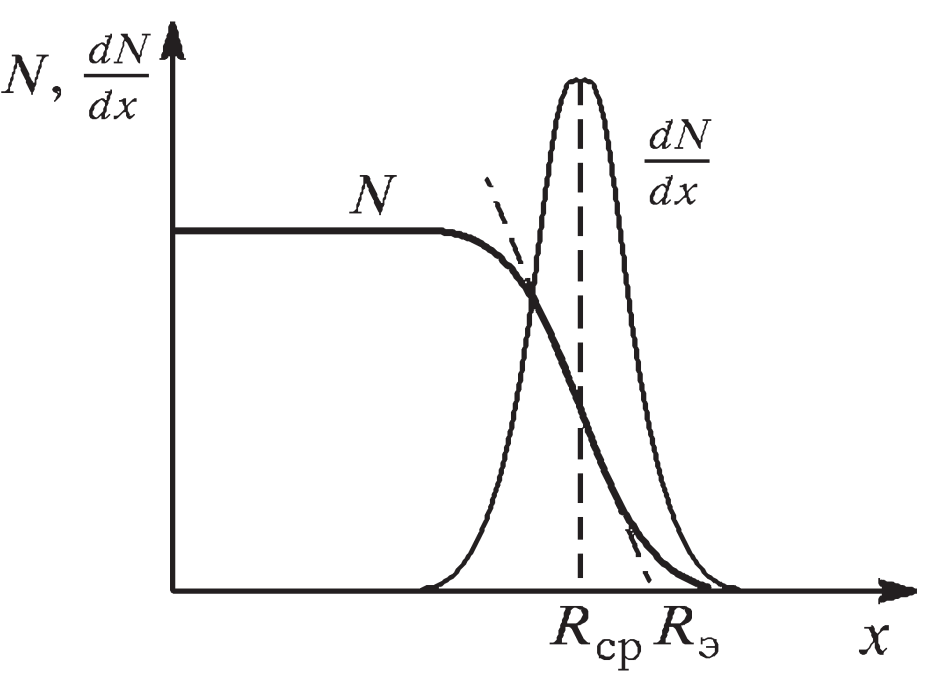
\includegraphics[width=0.45\textwidth]{Pictures/N(x)_theory}
		\caption{Зависимость числа $\alpha$-частиц от глубины их проникновения в вещество}
		\label{AlphaParticles_N(x)_theory}
	\end{wrapfigure}

	При малых глубинах число частиц не меняется с расстоянием. В конце пути это число не сразу обрывается до нуля, а приближается к нему постепенно. Как видно из кривой $dN/dx$, бóльшая часть $\alpha$-частиц останавливается в узкой области, расположенной около некоторого значения $x$, которое называется средним пробегом $R_\text{ср}$. Иногда вместо $R_\text{ср}$ измеряют экстраполированный пробег $R_\text{э}$. Чтобы его получить, нужно продолжить касательную к кривой $N(x)$, взятую в точке $x = R_\text{ср}$, до пересечения с осью $x$.
	
	Несмотря на наличие коллиматора, в данной работе мы имеем дело не с узкими параллельными пучками частиц, а с пучками конечных размеров, обладающими заметной угловой расходимостью. Это приводит к тому, что экспериментально наблюдаемые зависимости числа $\alpha$-частиц от глубины их проникновения качественно правильно передают появление брэгговского пика и, тем самым, относительную величину пробега частиц с разной энергией. Однако в силу указанных причин брэгговский пик оказывается смещенным и сильно размытым. Поэтому лучшей оценкой пробега оказывается экстраполированный пробег.

	
	\tocsection{Ход работы}
	
	\tocsubsection{Исследование пробега $\alpha$-частиц с помощью счетчика Гейгера}
	
	Для определения пробега $\alpha$-частиц с помощью счетчика радиоактивный источник помещается на дно стальной цилиндрической бомбы (рис. \ref{AlphaParticles_Geiger}), в которой может перемещаться торцевой счетчик Гейгера. Его чувствительный объем отделен от наружной среды тонким слюдяным окошком, сквозь которое могут проходить $\alpha$-частицы. 
	
	\begin{figure}[h!]
		\centering
		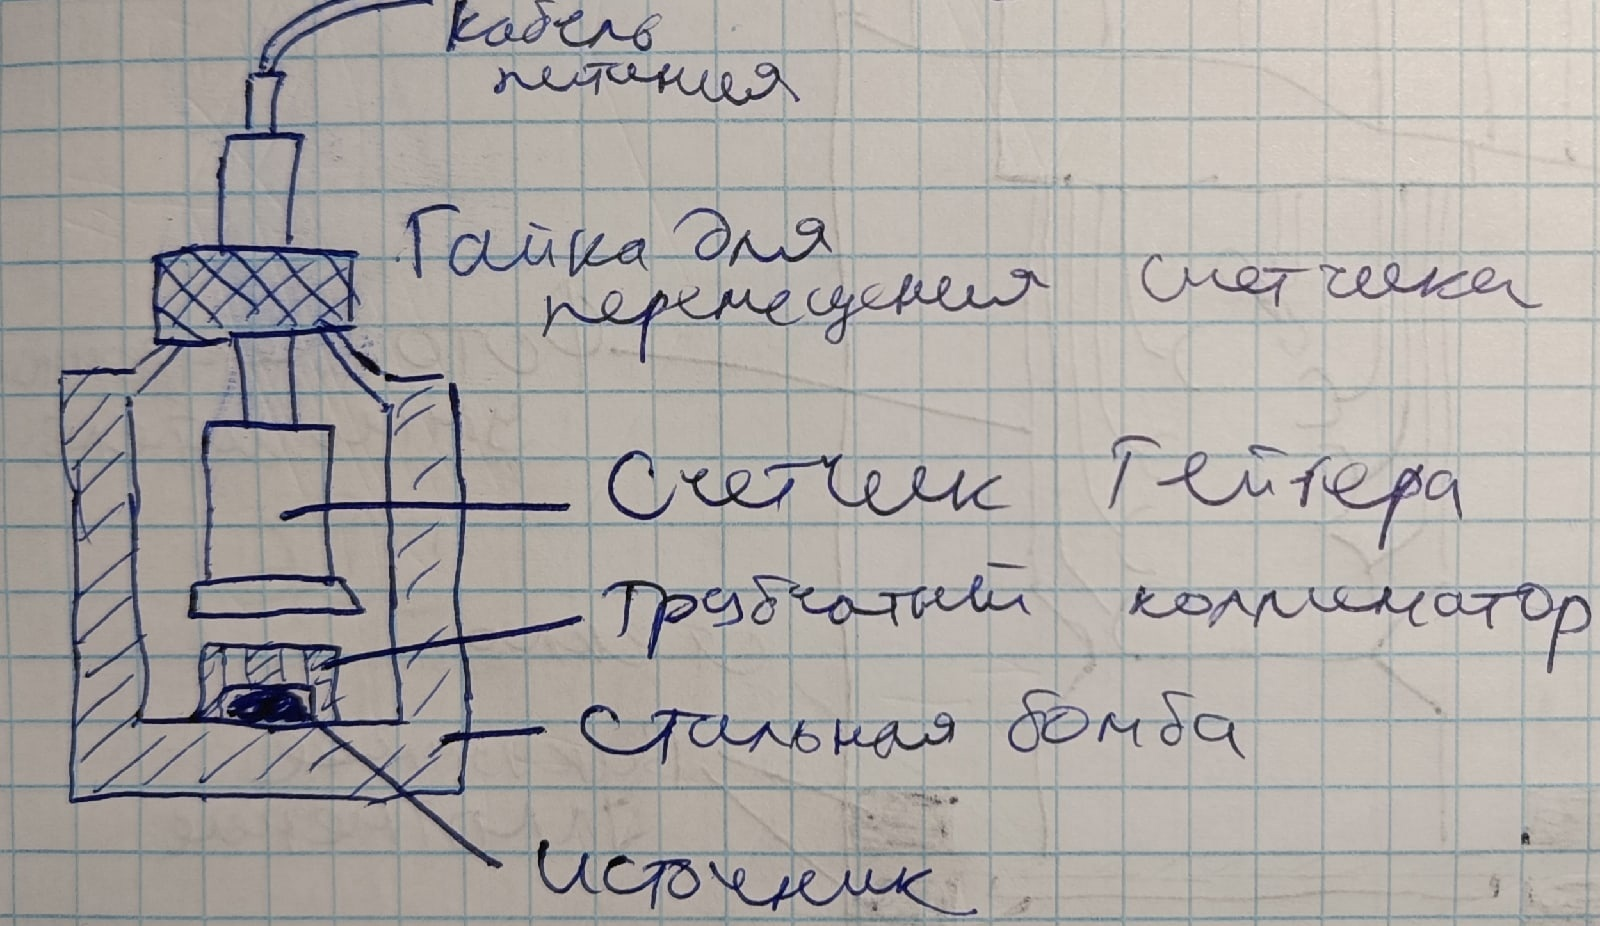
\includegraphics[width=\linewidth]{Pictures/Geiger}
		\caption{Установка для измерения пробега $\alpha$-частиц с помощью торцевого счетчика Гейгера}
		\label{AlphaParticles_Geiger}
	\end{figure}

	Импульсы, возникающие в счетчике, усиливаются и регистрируются пересчетной схемой. Путь частиц в воздухе зависит от расстояния между источником и счетчиком. Перемещение счетчика производится путем вращения гайки, находящейся на крышке бомбы.

	
	\begin{enumerate}
		\item Включим пересчетную установку и высоковольтный выпрямитель. 
		
		\item Проведем измерения зависимости скорости счета $N$ от расстояния $x$ между источником и счетчиком. Результаты пишем в таблицу \ref{AlphaParticles_N(x)}.

		\begin{table}[h!]
			\centering
				\begin{tabular}{|r|r|r|r|r|r|}
					\hline
					\multicolumn{1}{|c|}{$x$, мм} & \multicolumn{1}{c|}{$\sigma_x$, мм} & \multicolumn{1}{c|}{$N_0$} & \multicolumn{1}{c|}{$t$, с} & \multicolumn{1}{c|}{$N$, с$^{-1}$} & \multicolumn{1}{c|}{$\sigma_{N}$, с$^{-1}$} \\ \hline
					10                            & 0,5                                 & 149                        & 10,2                        & 14,61                              & 1,20                                         \\ \hline
					11                            & 0,5                                 & 453                        & 30,4                        & 14,90                              & 0,70                                         \\ \hline
					12                            & 0,5                                 & 638                        & 40,1                        & 15,91                              & 0,60                                         \\ \hline
					13                            & 0,5                                 & 685                        & 45,1                        & 15,19                              & 0,60                                         \\ \hline
					14                            & 0,5                                 & 600                        & 40,1                        & 14,96                              & 0,60                                         \\ \hline
					15                            & 0,5                                 & 430                        & 30,3                        & 14,19                              & 0,70                                         \\ \hline
					16                            & 0,5                                 & 646                        & 45,2                        & 14,29                              & 0,60                                         \\ \hline
					17                            & 0,5                                 & 605                        & 49,3                        & 12,27                              & 0,50                                         \\ \hline
					18                            & 0,5                                 & 217                        & 40,1                        & 5,41                               & 0,40                                         \\ \hline
					19                            & 0,5                                 & 57                         & 90,2                        & 0,63                               & 0,10                                         \\ \hline
					20                            & 0,5                                 & 16                         & 41,0                        & 0,39                               & 0,10                                         \\ \hline
					21                            & 0,5                                 & 26                         & 70,1                        & 0,37                               & 0,07                                        \\ \hline
					22                            & 0,5                                 & 18                         & 65,3                        & 0,28                               & 0,06                                        \\ \hline
					24                            & 0,5                                 & 17                         & 70,2                        & 0,24                               & 0,06                                        \\ \hline
					26                            & 0,5                                 & 14                         & 70,2                        & 0,20                               & 0,05                                        \\ \hline
					28                            & 0,5                                 & 13                         & 54,8                        & 0,24                               & 0,07                                        \\ \hline
					30                            & 0,5                                 & 15                         & 70,0                        & 0,21                               & 0,06                                        \\ \hline
				\end{tabular}
			\caption{Зависимость скорости счета от расстояния}
			\label{AlphaParticles_N(x)}
		\end{table}

	
		\item Построим график $N(x)$. Для этого попробуем аппроксимировать наш набор точек кривой вида
		\begin{equation*}
			N(x) = \frac{A}{1 + \exp{\left(\frac{x - x_0}{B}\right)}} + C.
		\end{equation*}
		Используя МНК, получаем следующие коэффициенты:
		\begin{itemize}
			\item $A = (14,7 \pm 0,2)$
			
			\item $B = (0,46 \pm 0,04) \text{ мм}$
			
			\item $C = (0,26 \pm 0,03)$
			
			\item $x_0 = (17,7 \pm 0,5) \text{ мм}$
		\end{itemize}
	
		Также, чтобы проанализировать производную $dN/dx$, построим график $-2\dfrac{dN}{dx}(x)$.
		
		Помимо этого, построим график $N(x)$ с аппроксимацией центральной части, чтобы найти $R_\text{э}$ как пересечение линейной экстраполяции до пересечения с осью абсцисс.
		
	
		\begin{figure}[h!]
			\centering
			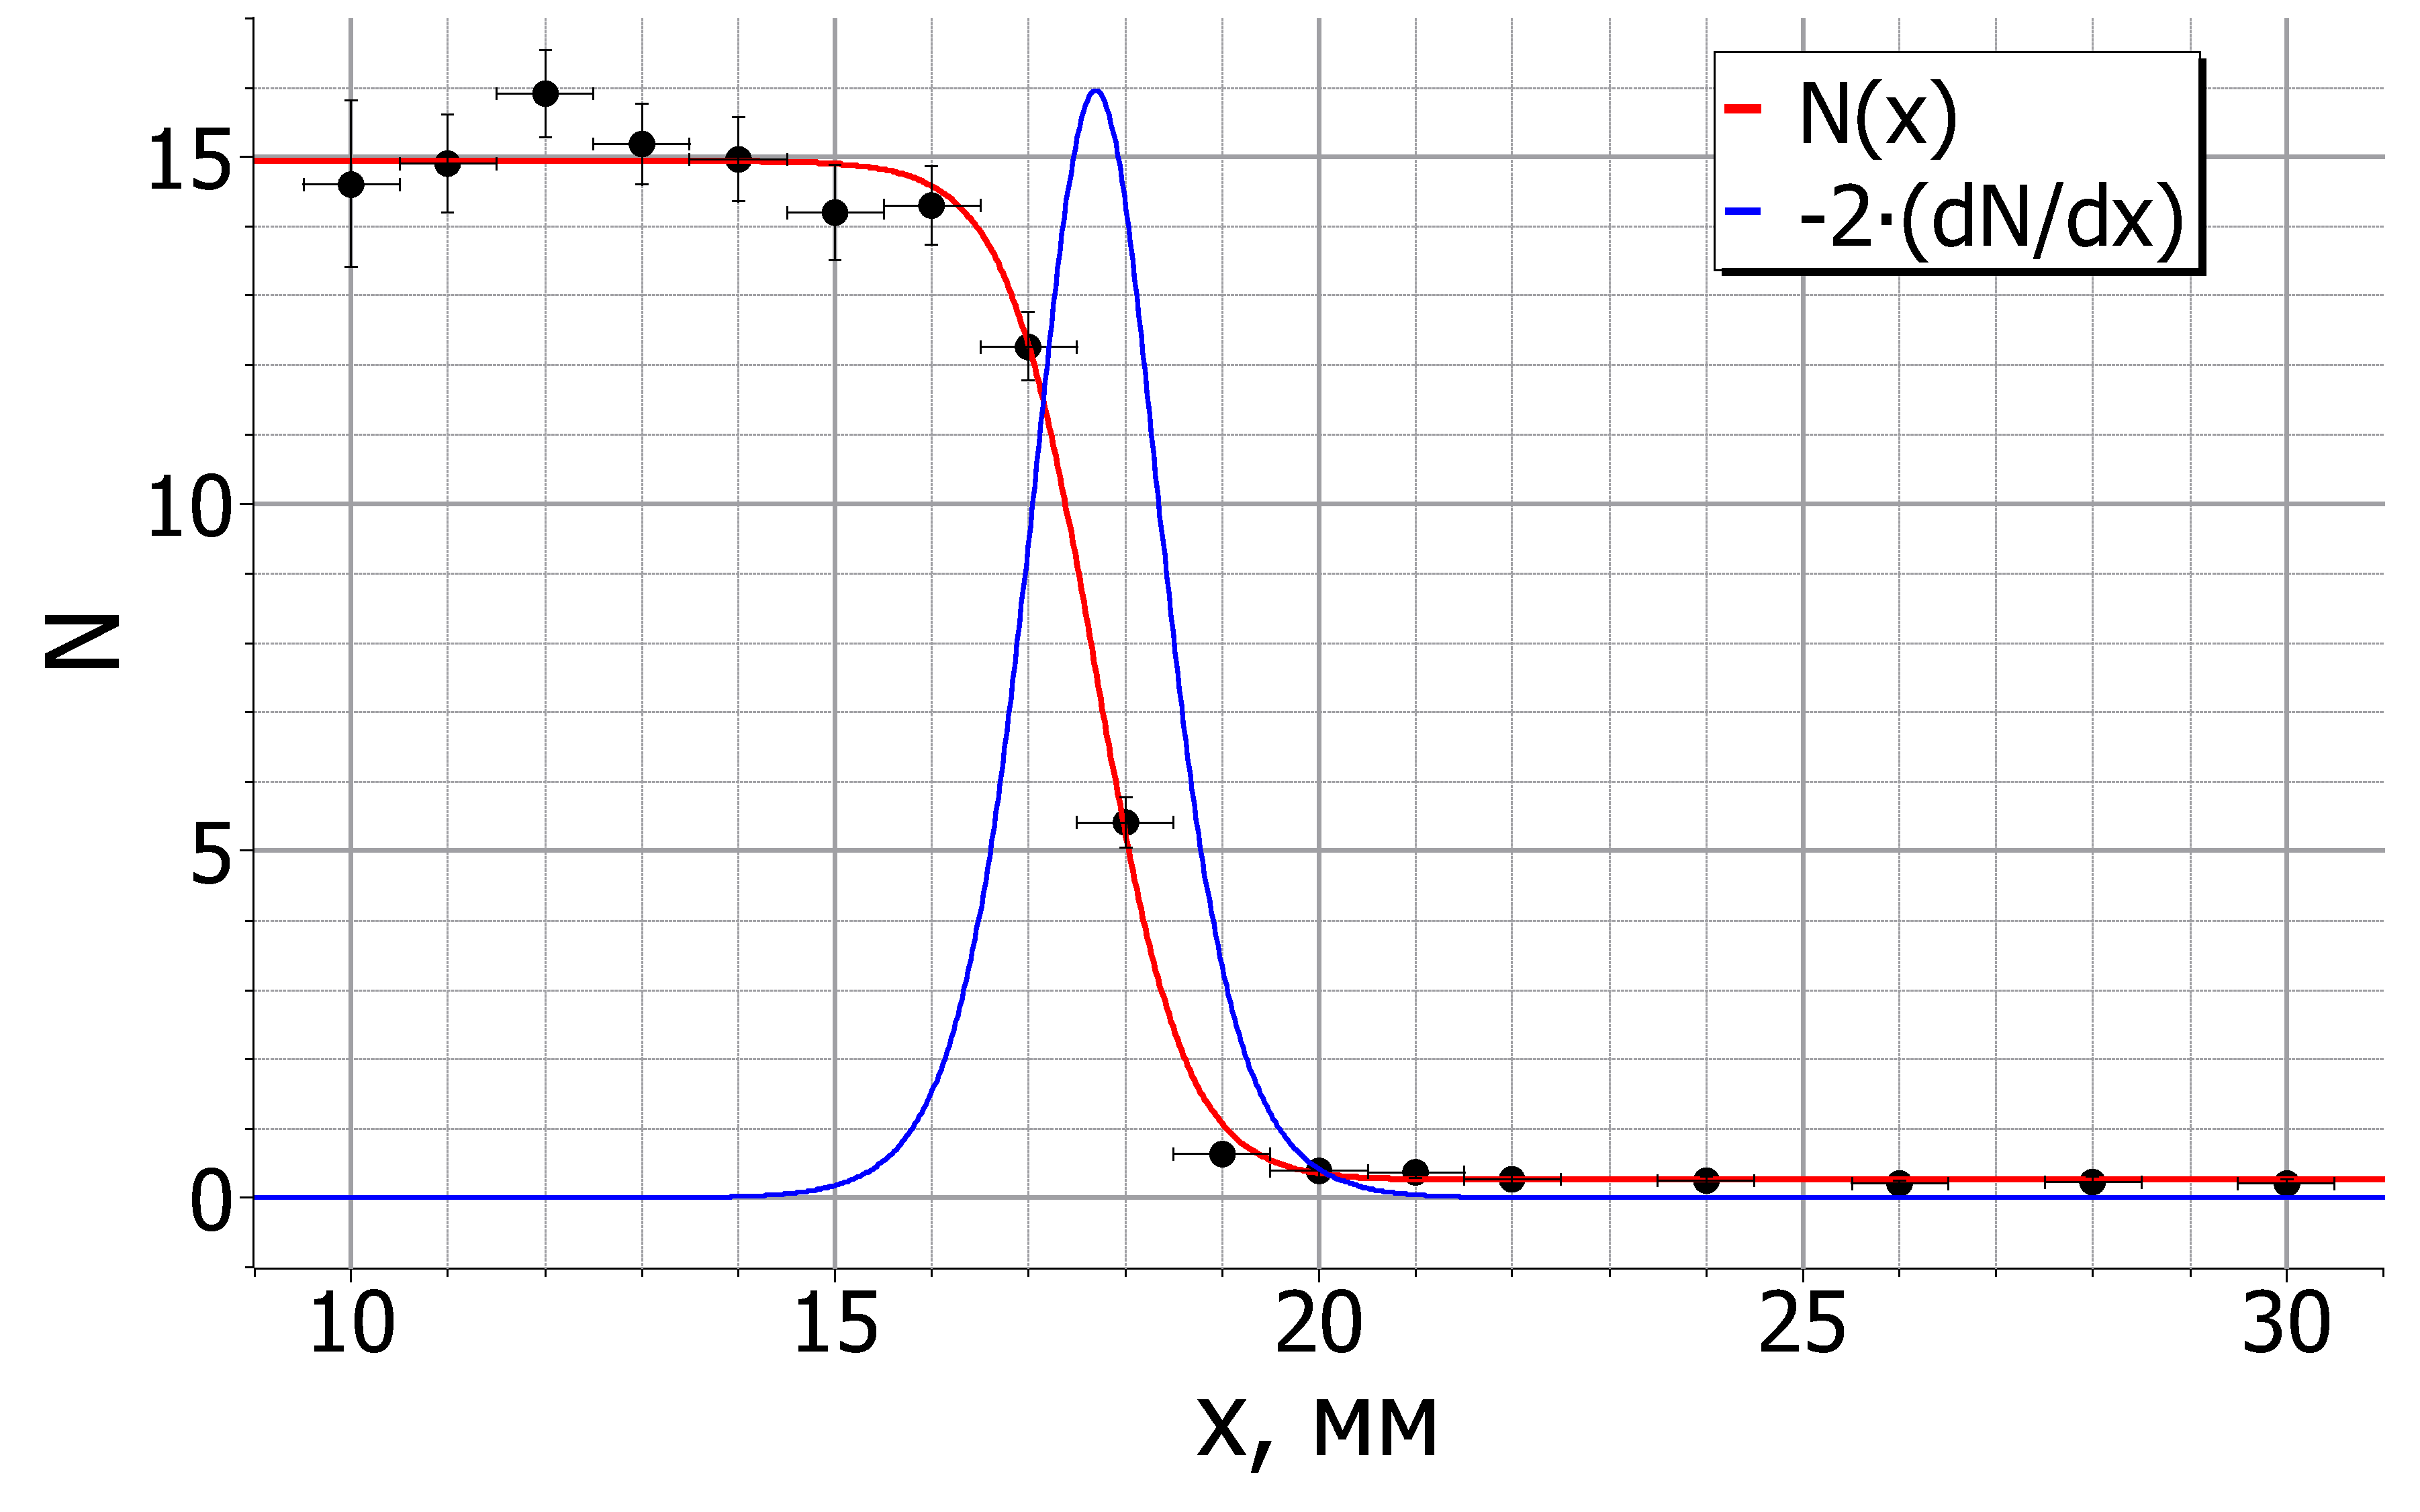
\includegraphics[width=0.98\linewidth]{Pictures/Geiger_PlotNoFit.pdf}
			\caption{График зависимости $N(x)$}
		\end{figure}
		
		\begin{figure}[h!]
			\centering
			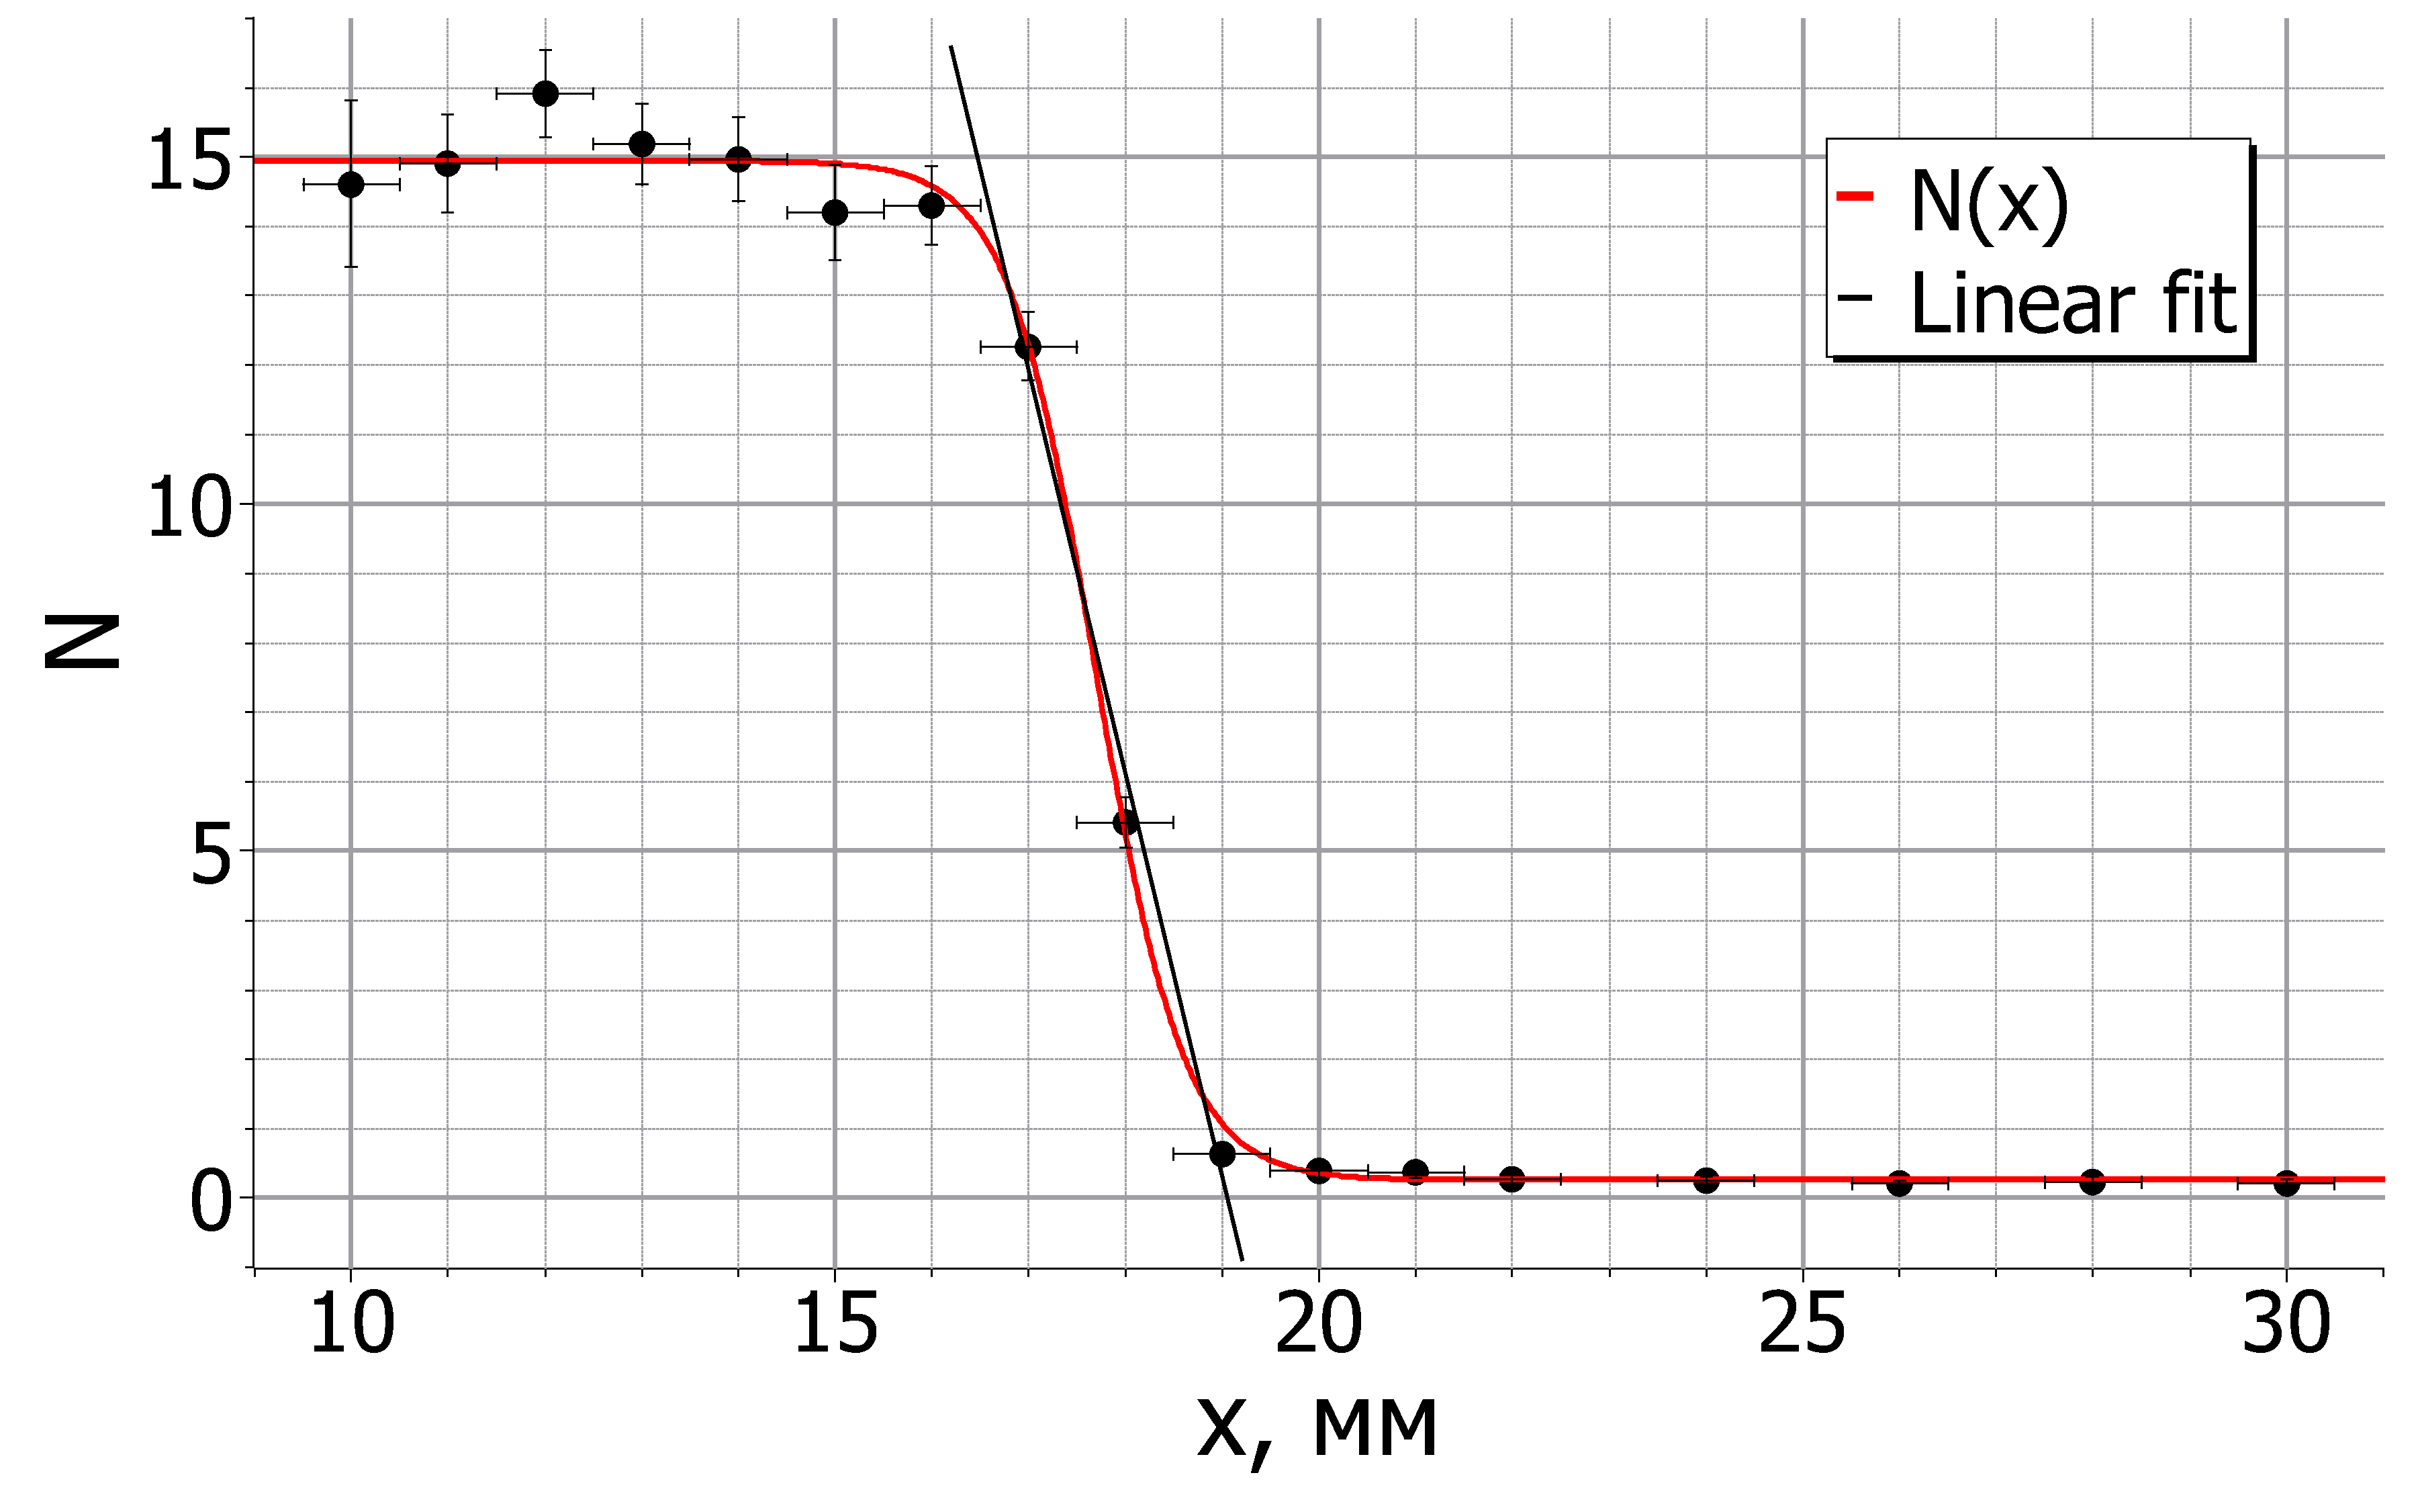
\includegraphics[width=0.98\linewidth]{Pictures/Geiger_PlotFit.pdf}
			\caption{График зависимости $N(x)$ с аппроксимацией центральной части}
		\end{figure}
		
		
		
		Из графиков получаем:
		\begin{itemize}
			\item $R_\text{ср} = x_0 = (17,7 \pm 0,5) \text{ мм} = (1,77 \pm 0,05) \text{ см}$;
			
			
			\item $R_\text{э} \,\, = (19 \pm 3) \text{ мм} = (1,9 \pm 0,3) \text{ см}$.
		\end{itemize}
	
		При плотности воздуха $\rho = 1,17 \cdot 10^{-3} \;\dfrac{\text{г}}{\text{см}^3}$ ($P = 99,3 \text{ кПа}$, $t = 22\;^\circ \text{C}$):
		\begin{itemize}
			\item $R'_\text{ср} = (2,07 \pm 0,06) \cdot 10^{-3} \;\dfrac{\text{г}}{\text{см}^2}$;
			
			
			\item $R'_\text{э} \,\, = (2,2 \pm 0,4) \cdot 10^{-3} \;\dfrac{\text{г}}{\text{см}^2}$.
		\end{itemize}
	
		Для энергий получаем:
		\begin{itemize}
			\item $E_\text{ср} = (3,13 \pm 0,06) \text{ МэВ}$;
			
			\item $E_\text{э} \,\, = (3,3 \pm 0,4) \text{ МэВ}$.
		\end{itemize}
	
	Как видим, результаты совпадают по порядку с истинным значением $E = 5,15$ МэВ, однако только лишь по нему и совпадают. Объясняется такое расхождение тем, что часть энергии $\alpha$-частиц тратится на преодоление слюдяной пластинки.
	
	\end{enumerate}
	
	\newpage
	\tocsubsection{Определение пробега $\alpha$-частиц сцинтилляционным счетчиком}
	
	\begin{wrapfigure}{R}{0.5\textwidth}
		\centering
		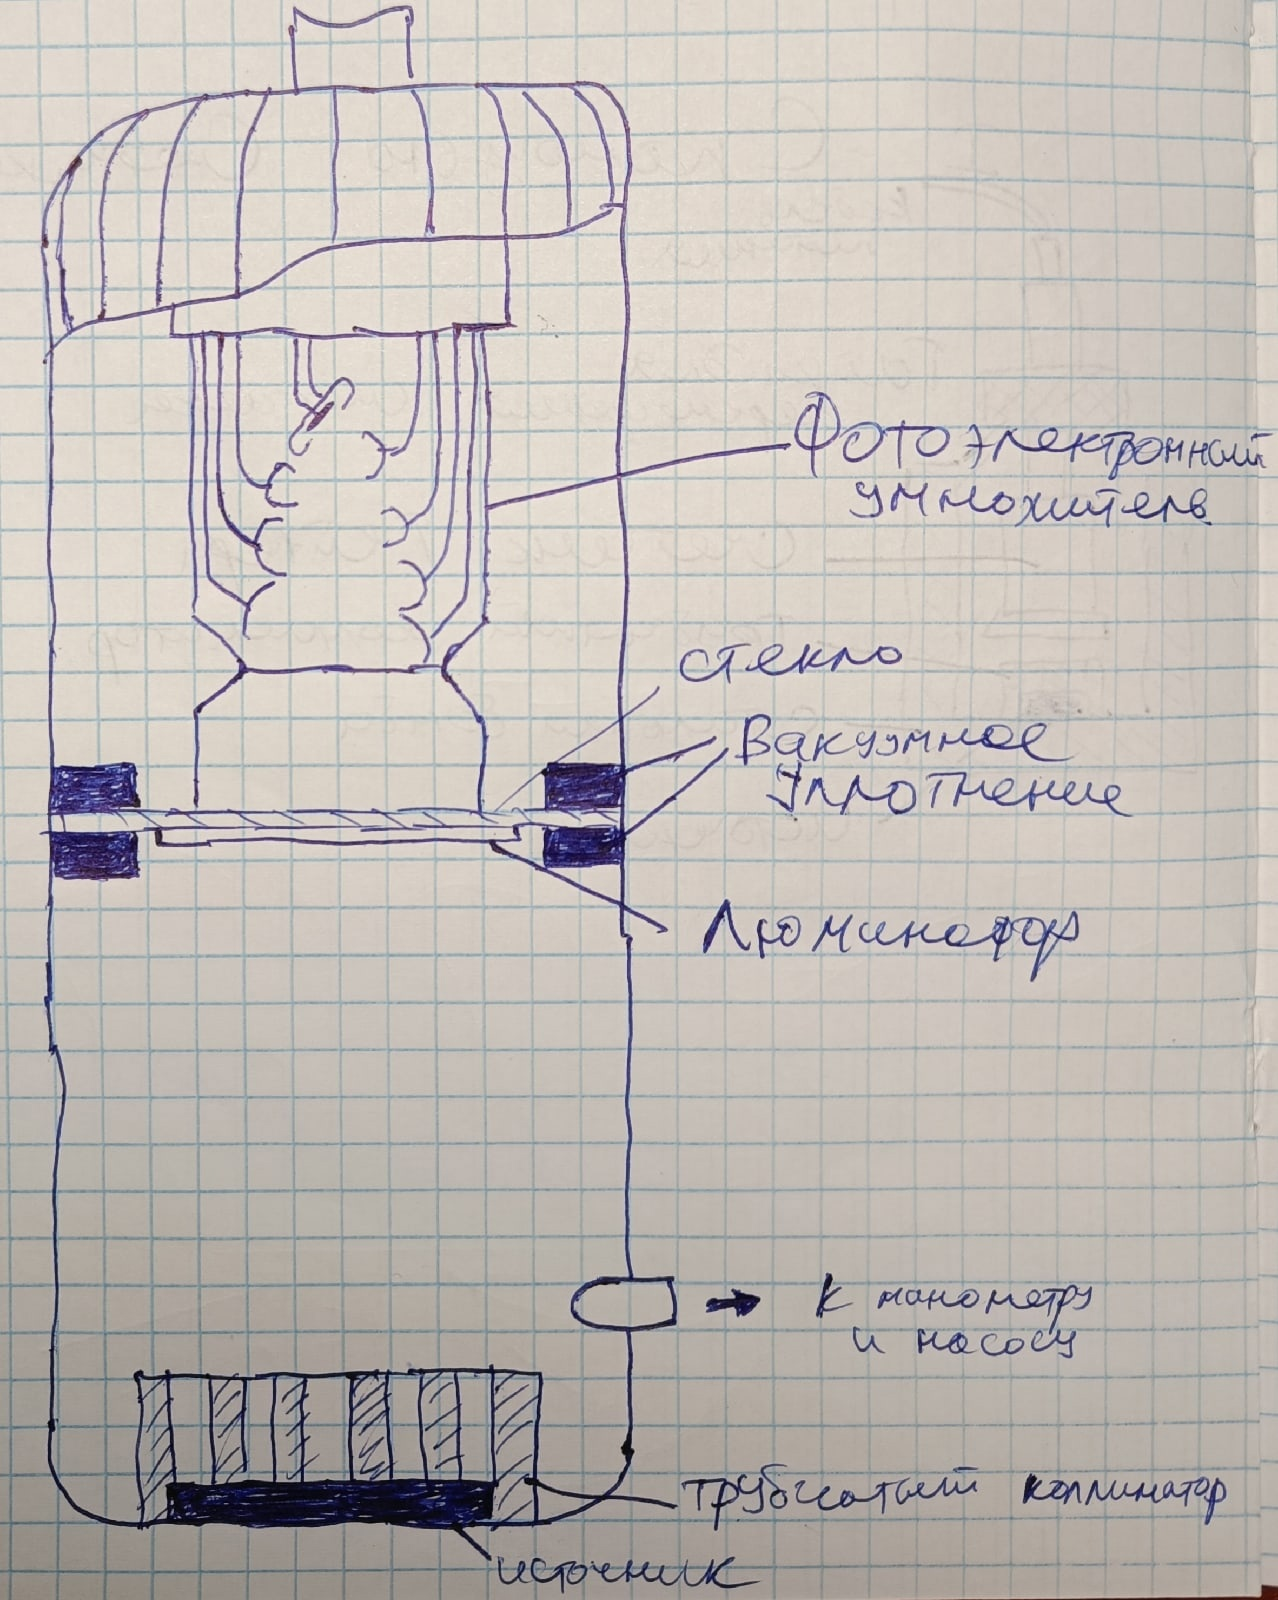
\includegraphics[width=0.45\textwidth]{Pictures/ScintillationChamber}
		\caption{Установка для измерения пробега $\alpha$-частиц с помощью сцинтилляционного счетчика}
		\label{AlphaParticles_ScintillationChamber}
	\end{wrapfigure}
	
	
	Установка состоит из цилиндрической камеры, на дне которой находится исследуемый препарат. Камера герметично закрыта стеклянной пластинкой, на которую с внутренней стороны нанесен слой люминофора. С наружной стороны к стеклу прижат фотокатод фотоумножителя (рис. \ref{AlphaParticles_ScintillationChamber}). Оптический контакт ФЭУ–стекло обеспечивается тонким слоем вазелинового масла.

	Сигналы с фотоумножителя через усилитель поступают на пересчетную установку. Рабочее напряжение фотоумножителя указано на высоковольтном выпрямителе. Определение пробега сводится к измерению зависимости интенсивности счета от давления в камере.
	
	\begin{enumerate}
		\item Включим пересчетную установку и высоковольтный выпрямитель.
		
		\item Проведем измерения зависимости счета $N$ от давления $P$ в камере. Результаты занесем в таблицу \ref{AlphaParticles_N(P)}.
		
		\item Построим график зависимости $N(P)$.
		
		\newpage
		\begin{table}[h!]
			\centering
				\begin{tabular}{|r|r|r|r|r|r|}
					\hline
					\multicolumn{1}{|c|}{$P_\text{изм}$, торр} & \multicolumn{1}{c|}{$P = P_0 - P_\text{изм}$, торр} & \multicolumn{1}{c|}{$N_0$} & \multicolumn{1}{c|}{$t$, с} & \multicolumn{1}{c|}{$N$, c$^{-1}$} & \multicolumn{1}{c|}{$\sigma_N$, c$^{-1}$} \\ \hline
					0                                                 & 745                                                        & 2                          & 10                          & 0,2                                & 0,2                                       \\ \hline
					100                                               & 645                                                        & 6                          & 10                          & 0,6                                & 0,3                                       \\ \hline
					150                                               & 595                                                        & 3                          & 10                          & 0,3                                & 0,2                                       \\ \hline
					200                                               & 545                                                        & 5                          & 10                          & 0,5                                & 0,2                                       \\ \hline
					350                                               & 395                                                        & 2                          & 10                          & 0,2                                & 0,2                                       \\ \hline
					400                                               & 345                                                        & 2                          & 10                          & 0,2                                & 0,2                                       \\ \hline
					450                                               & 295                                                        & 38                         & 10                          & 3,8                                & 0,6                                       \\ \hline
					480                                               & 265                                                        & 95                         & 10                          & 7,2                                & 0,8                                       \\ \hline
					500                                               & 245                                                        & 97                         & 10                          & 9,7                                & 1,0                                       \\ \hline
					510                                               & 235                                                        & 115                        & 10                          & 11,5                               & 1,0                                       \\ \hline
					535                                               & 210                                                        & 222                        & 10                          & 22,2                               & 2,0                                       \\ \hline
					550                                               & 195                                                        & 401                        & 10                          & 40,1                               & 2,0                                       \\ \hline
					580                                               & 165                                                        & 722                        & 10                          & 72,2                               & 3,0                                       \\ \hline
					590                                               & 155                                                        & 996                        & 10                          & 99,6                               & 3,0                                       \\ \hline
					600                                               & 145                                                        & 1182                       & 10                          & 118,2                              & 4,0                                       \\ \hline
					640                                               & 105                                                        & 1967                       & 10                          & 196,7                              & 5,0                                       \\ \hline
					650                                               & 95                                                         & 2309                       & 10                          & 230,9                              & 5,0                                       \\ \hline
					675                                               & 70                                                         & 2877                       & 10                          & 287,7                              & 5,0                                       \\ \hline
					700                                               & 45                                                         & 3123                       & 10                          & 312,3                              & 6,0                                       \\ \hline
					730                                               & 15                                                         & 3516                       & 10                          & 351,6                              & 6,0                                       \\ \hline
					735                                               & 10                                                         & 3544                       & 10                          & 354,4                              & 6,0                                       \\ \hline
				\end{tabular}
			\caption{Зависимость $N(P)$}
			\label{AlphaParticles_N(P)}
		\end{table}
	
	
		\begin{figure}[h!]
			\centering
			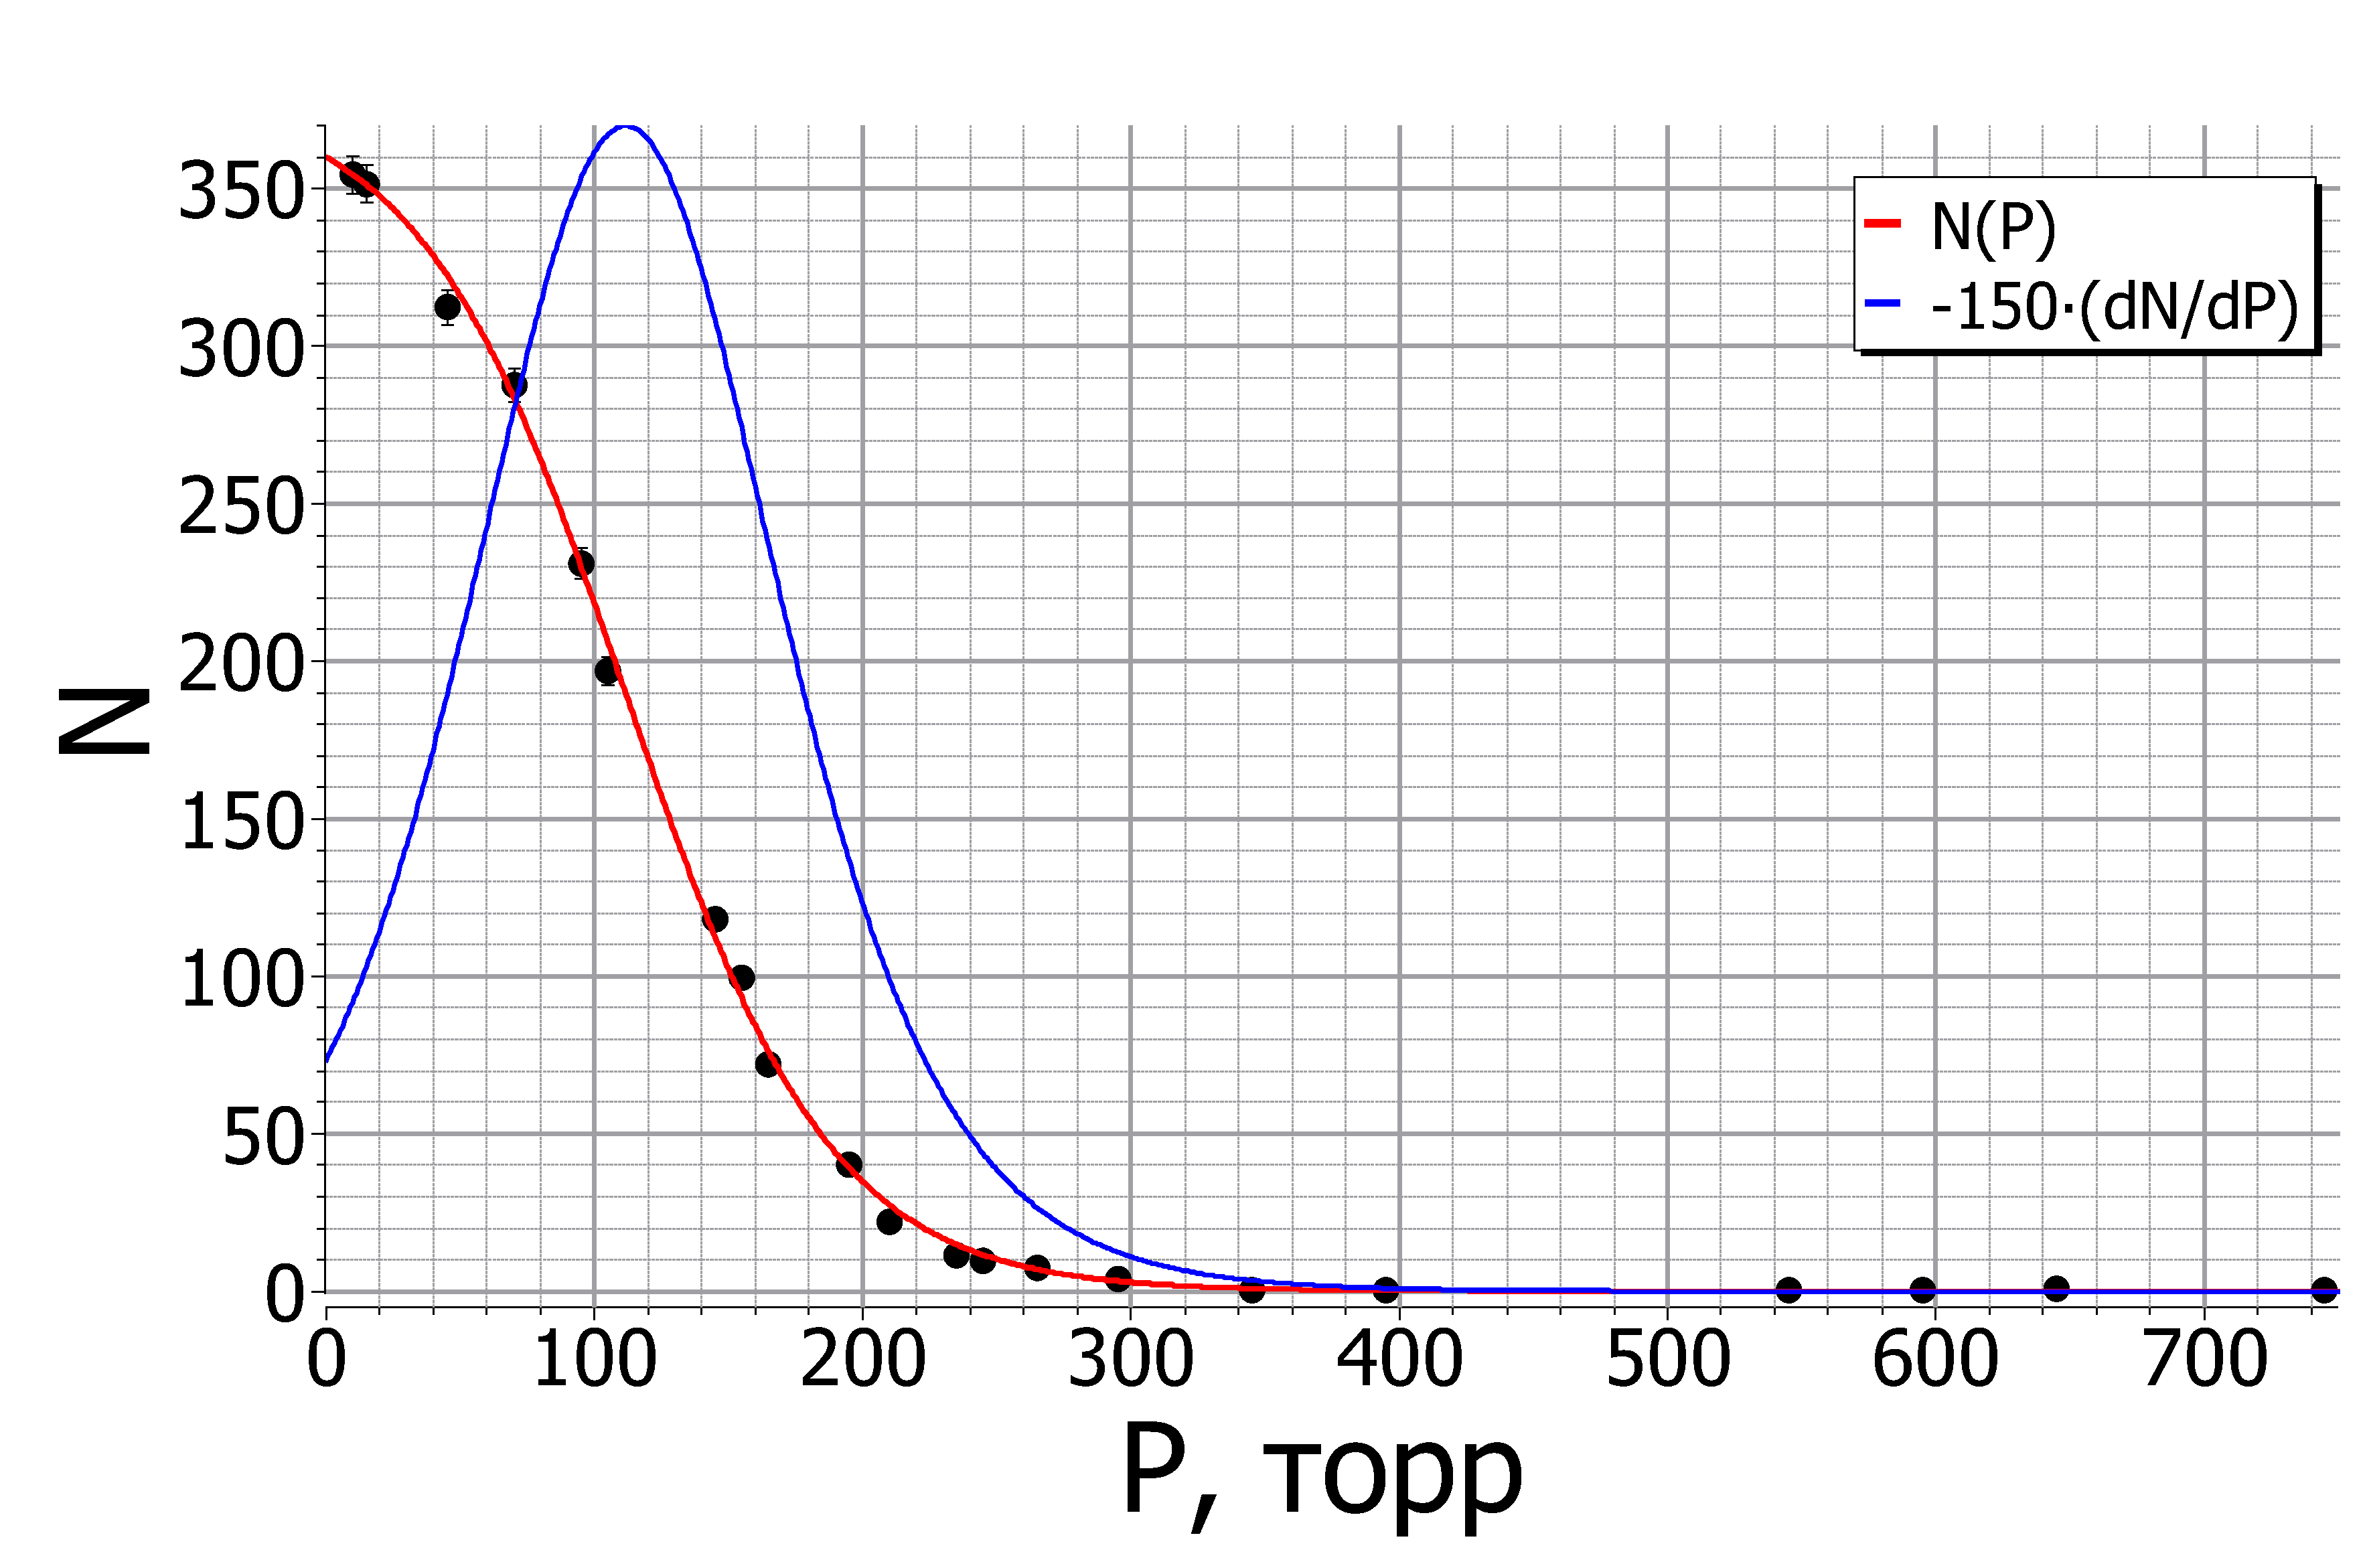
\includegraphics[width=\linewidth]{Pictures/Scintillation_PlotNoFit.pdf}
			\caption{Зависимость $N(x)$}
		\end{figure}
	
		\begin{figure}[h!]
			\centering
			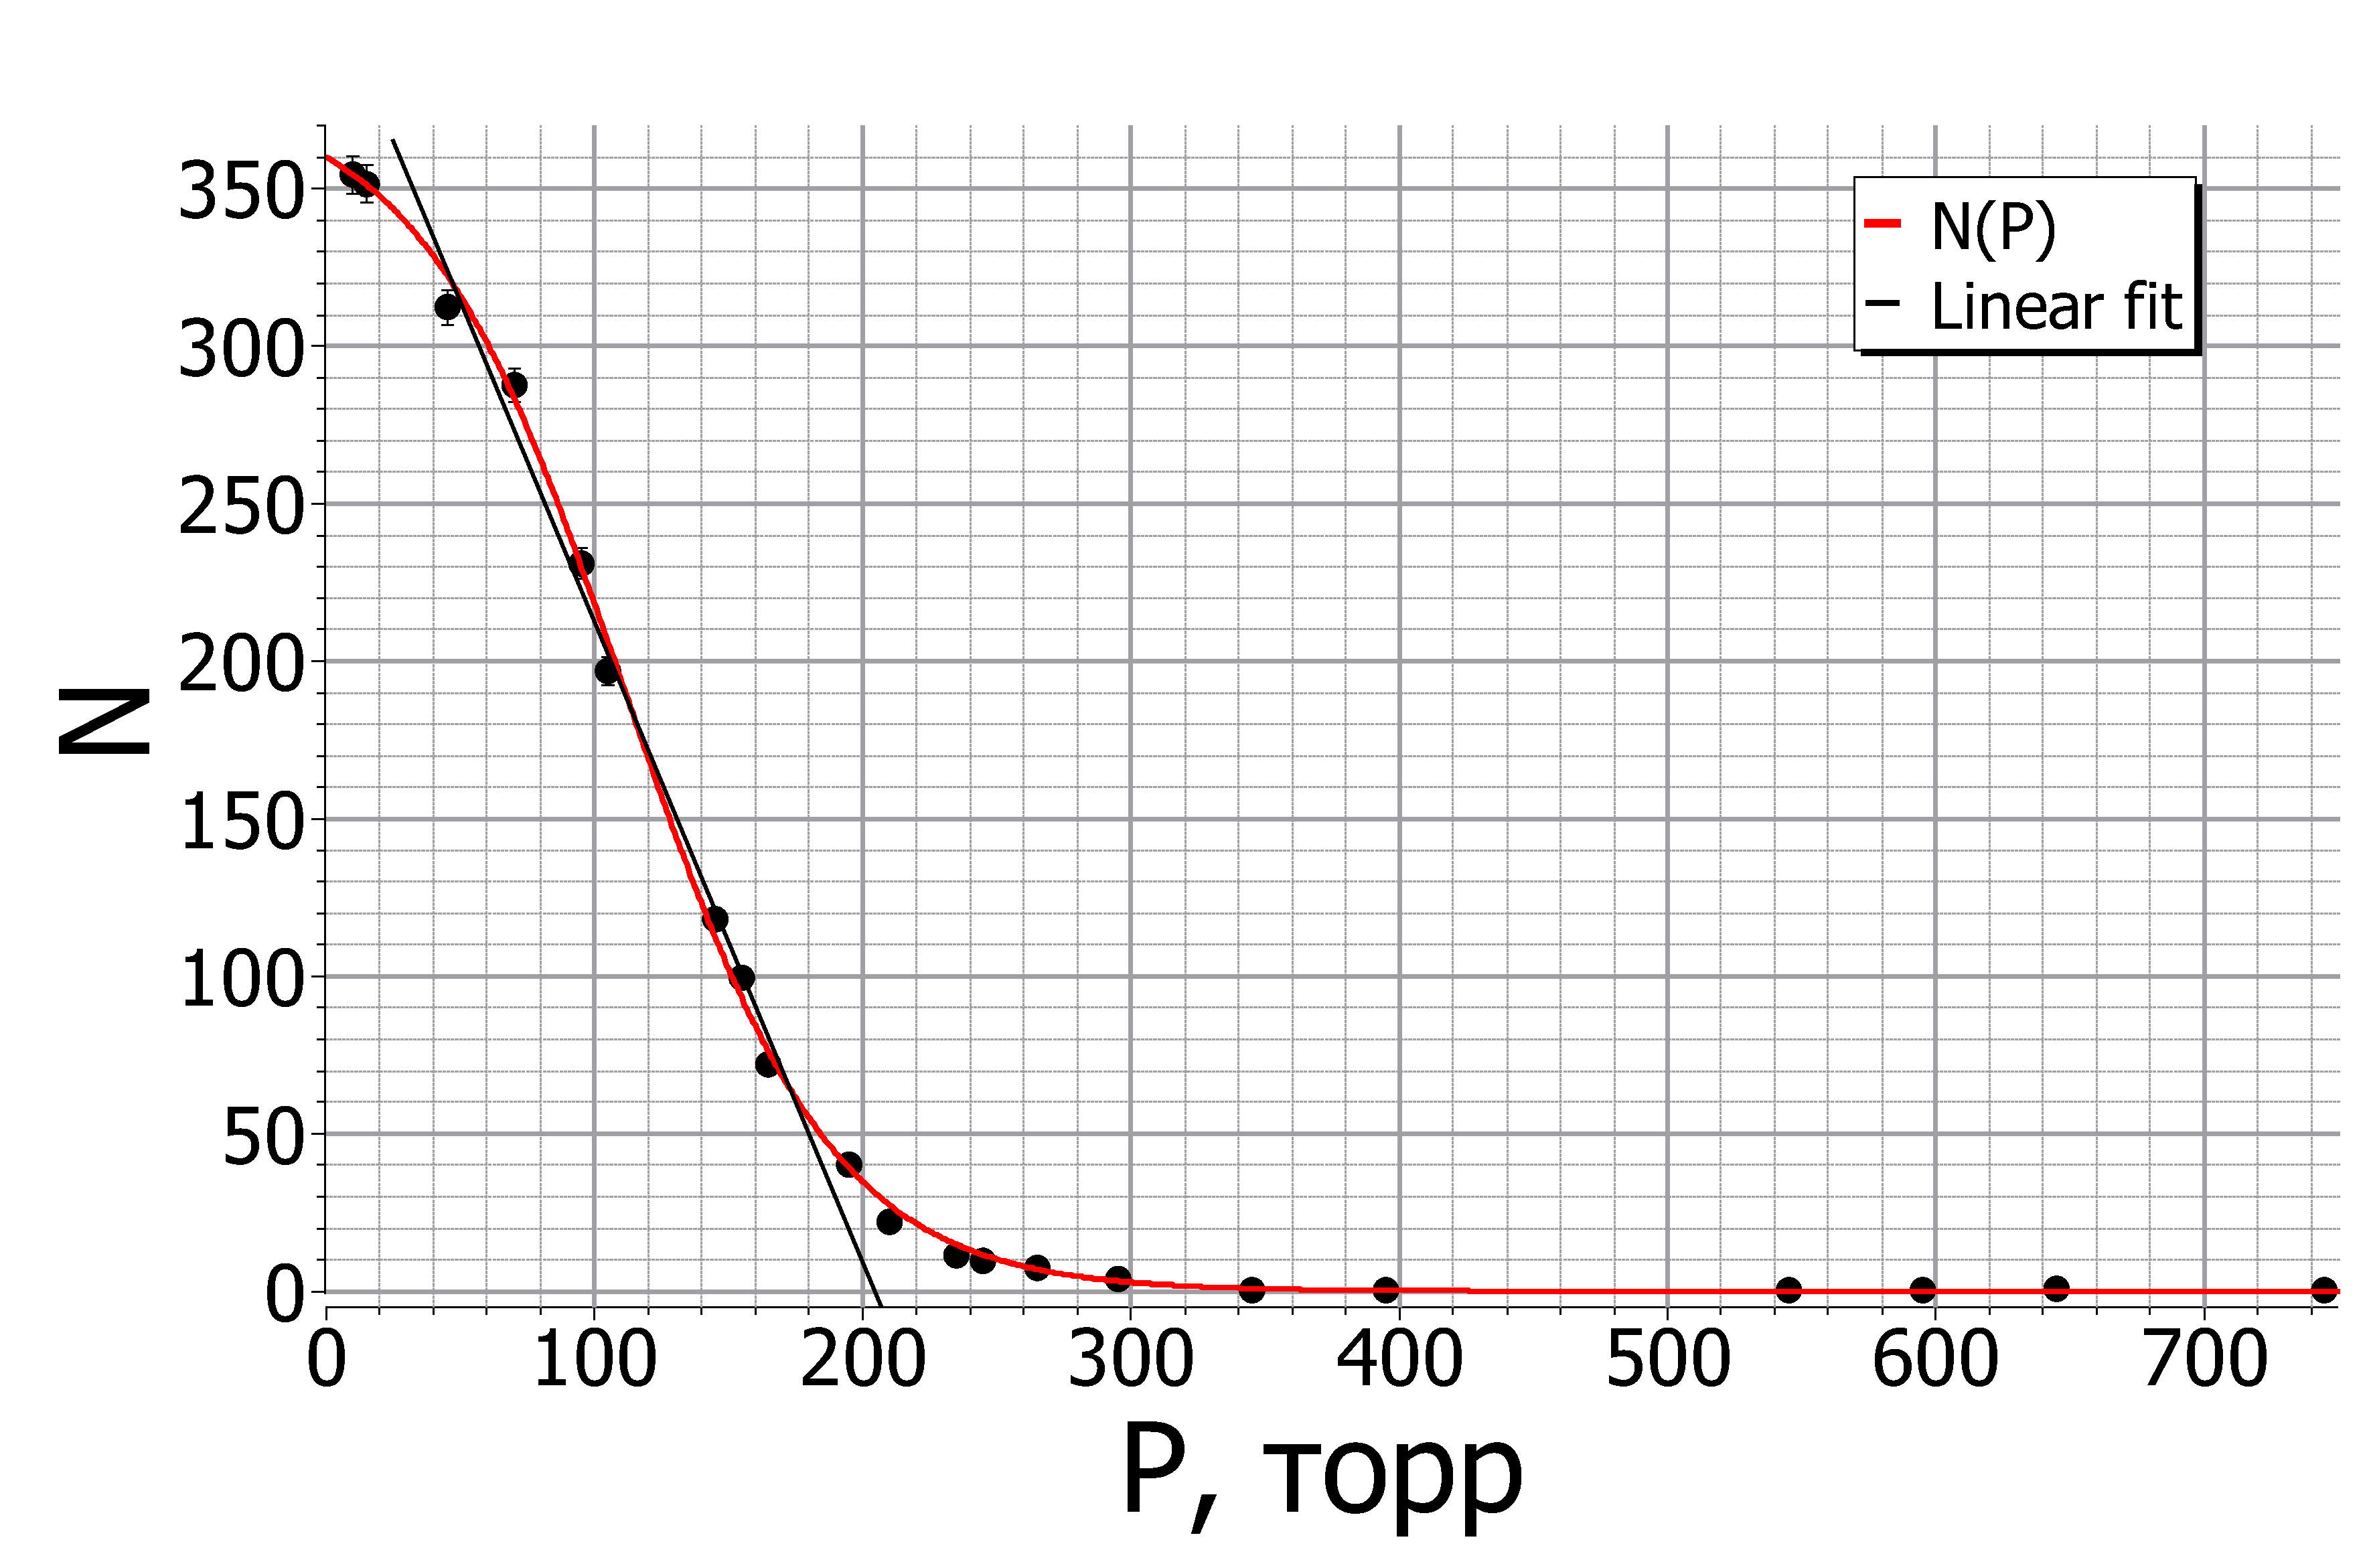
\includegraphics[width=\linewidth]{Pictures/Scintillation_PlotFit.pdf}
			\caption{Зависимость $N(x)$ с аппроксимацией центральной части}
		\end{figure}
	
	
		\newpage
		Из графиков получаем:
		\begin{itemize}
			\item $P_\text{ср} = (112 \pm 4) \text{ торр}$;
			
			
			\item $P_\text{э} \,\, = (204 \pm 13) \text{ торр}$.
		\end{itemize}
	
		Это давление, при котором длина свободного пробега равна расстоянию от источника для люминофора $L = 9$ см. 
		
		Пересчитаем длину свободного пробега для нормальных условий ($P = 760$ торр, $t = 15$ $^\circ$C):
		\begin{equation*}
			R_\text{э} = L\frac{P_\text{э}}{P_0}, 
		\end{equation*}
		\noindent где $P_0 = 760$ торр. Тогда:
		
		\begin{itemize}
			\item $R_\text{ср} = (1,32 \pm 0,05) \text{ см}$;
			
			
			\item $R_\text{э} \,\, = (2,4 \pm 0,2) \text{ см}$.
		\end{itemize}
		
		При плотности воздуха $\rho = 1,17 \cdot 10^{-3} \;\dfrac{\text{г}}{\text{см}^3}$ ($P = 99,3 \text{ кПа}$, $t = 22\;^\circ \text{C}$):
		\begin{itemize}
			\item $R'_\text{ср} = (1,55 \pm 0,06) \cdot 10^{-3} \;\dfrac{\text{г}}{\text{см}^2}$;
			
			
			\item $R'_\text{э} \,\, = (2,8 \pm 0,2) \cdot 10^{-3} \;\dfrac{\text{г}}{\text{см}^2}$.
		\end{itemize}
		
		Для энергий получаем:
		\begin{itemize}
			\item $E_\text{ср} = (2,9 \pm 0,1) \text{ МэВ}$;
			
			\item $E_\text{э} \,\, = (3,8 \pm 0,2) \text{ МэВ}$.
		\end{itemize}
	
		Опять же, результаты совпадают по порядку с истинным значением. Однако они все еще не очень точны, хотя значение, полученное экстраполяцией, ближе этим методом, ближе всего к действительному значению. 
	\end{enumerate}

	\newpage
	\tocsubsection{ Определение пробега $\alpha$-частиц с помощью ионизационной камеры}
	
	\begin{wrapfigure}{R}{0.5\textwidth}
		\centering
		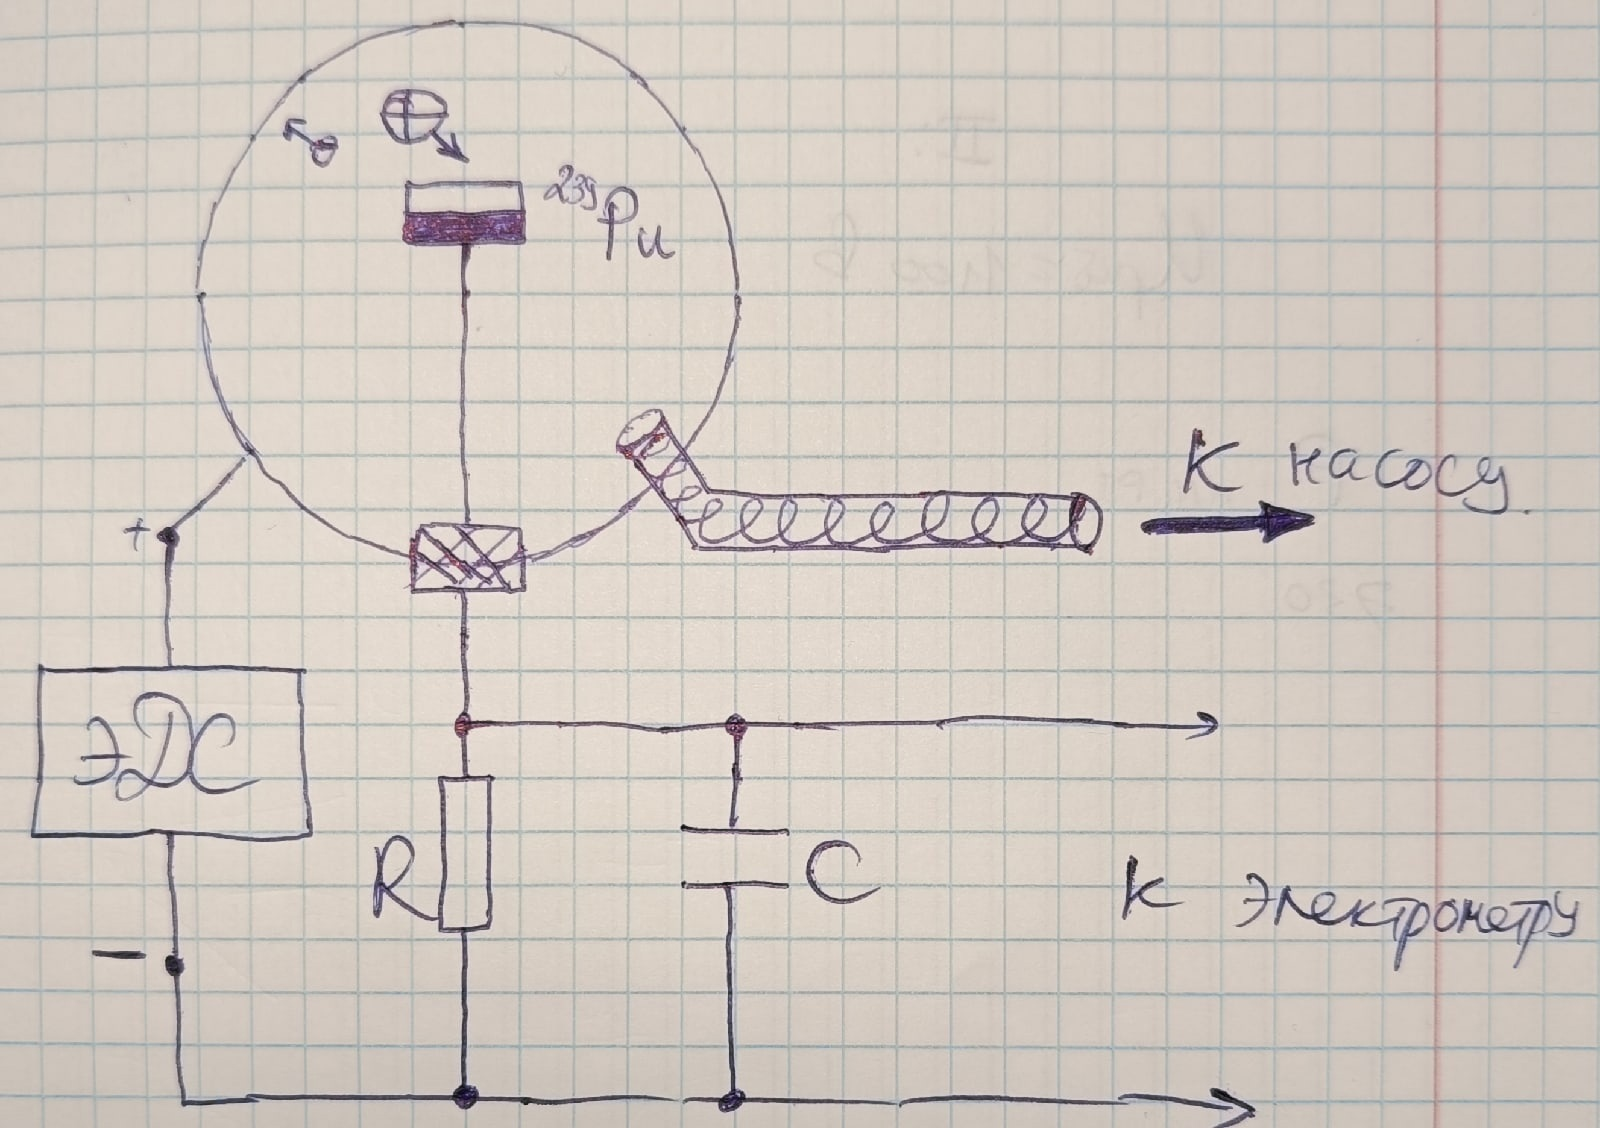
\includegraphics[width=0.45\textwidth]{Pictures/IonizationChamber}
		\caption{Схема устройства ионизационной камеры}
		\label{AlphaParticles_IonizationChamber}
	\end{wrapfigure}

	Ионизационная камера — прибор для количественного измерения ионизации, произведенной заряженными частицами при прохождении через газ. Камера представляет собой наполненный газом сосуд с двумя электродами (схема камеры приведена на рис.\ref{AlphaParticles_IonizationChamber}).Сферическая стенка прибора служит одним из электродов, второй электрод вводится в газ через изолирующую пробку. К электродам подводится постоянное напряжение от источника ЭДС.

	
	Заполняющий сосуд газ сам по себе не проводит электрический ток, возникает он только при прохождении быстрой заряженной частицы, которая рождает в газе на своем пути ионы.

	
	Ток, протекающий через камеру, вначале будет резко возрастать, а затем, начиная с некоторого напряжения $V_0$, станет постоянным, то есть выйдет на плато.
	
	Прохождение тока через камеру регистрируется посредством измерения напряжения на включенном в цепь камеры сопротивлении $R$.

	В данной работе измерение пробега $\alpha$-частицы проводится по величине тока ионизации в сферической камере. Разность потенциалов между электродами составляет 300 В. Вакуумная установка содержит кран и манометр. Она позволяет изменять давление в камере от атмосферного до 10 торр. Величина тока ионизации измеряется электрометром, состоящим из нескольких стандартных микросхем, по величине падения напряжения на сопротивлении $R = 100$ МОм. Значение измеряемого ионизационного тока высвечивается на цифровом табло.

	
	\begin{enumerate}
		\item Включим установку в сеть. Запишем значение <<нулевого>> показания табло: $I_0 = 19$ пА.
		
		\item Включим питание ионизационной камеры.
		
		\item Проведем измерения зависимости тока от давления. Результаты запишем в таблицу \ref{AlphaParticles_I(P)}.
	
		\newpage
		\begin{table}[h!]
			\centering
				\begin{tabular}{|r|r|rll|r|r|rll|r|r|}
					\cline{1-2} \cline{6-7} \cline{11-12}
					\multicolumn{1}{|r|}{$P$, торр} & \multicolumn{1}{r|}{$I$, пА} &  &  &  & \multicolumn{1}{r|}{$P$, торр} & \multicolumn{1}{r|}{$I$, пА} &  &  &  & \multicolumn{1}{r|}{$P$, торр} & \multicolumn{1}{r|}{$I$, пА} \\ \cline{1-2} \cline{6-7} \cline{11-12} 
					40                              & 22                           &  &  &  & 245                            & 329                          &  &  &  & 455                            & 742                          \\ \cline{1-2} \cline{6-7} \cline{11-12} 
					45                              & 26                           &  &  &  & 255                            & 343                          &  &  &  & 465                            & 759                          \\ \cline{1-2} \cline{6-7} \cline{11-12} 
					55                              & 27                           &  &  &  & 265                            & 374                          &  &  &  & 475                            & 782                          \\ \cline{1-2} \cline{6-7} \cline{11-12} 
					65                              & 36                           &  &  &  & 275                            & 389                          &  &  &  & 485                            & 797                          \\ \cline{1-2} \cline{6-7} \cline{11-12} 
					75                              & 52                           &  &  &  & 285                            & 403                          &  &  &  & 495                            & 814                          \\ \cline{1-2} \cline{6-7} \cline{11-12} 
					85                              & 62                           &  &  &  & 295                            & 429                          &  &  &  & 505                            & 831                          \\ \cline{1-2} \cline{6-7} \cline{11-12} 
					95                              & 74                           &  &  &  & 305                            & 449                          &  &  &  & 515                            & 849                          \\ \cline{1-2} \cline{6-7} \cline{11-12} 
					105                             & 83                           &  &  &  & 315                            & 465                          &  &  &  & 525                            & 864                          \\ \cline{1-2} \cline{6-7} \cline{11-12} 
					115                             & 93                           &  &  &  & 325                            & 475                          &  &  &  & 535                            & 884                          \\ \cline{1-2} \cline{6-7} \cline{11-12} 
					125                             & 127                          &  &  &  & 335                            & 495                          &  &  &  & 545                            & 912                          \\ \cline{1-2} \cline{6-7} \cline{11-12} 
					135                             & 140                          &  &  &  & 345                            & 519                          &  &  &  & 555                            & 932                          \\ \cline{1-2} \cline{6-7} \cline{11-12} 
					145                             & 154                          &  &  &  & 355                            & 546                          &  &  &  & 575                            & 964                          \\ \cline{1-2} \cline{6-7} \cline{11-12} 
					155                             & 169                          &  &  &  & 365                            & 561                          &  &  &  & 595                            & 982                          \\ \cline{1-2} \cline{6-7} \cline{11-12} 
					165                             & 197                          &  &  &  & 375                            & 594                          &  &  &  & 615                            & 994                          \\ \cline{1-2} \cline{6-7} \cline{11-12} 
					175                             & 211                          &  &  &  & 385                            & 608                          &  &  &  & 635                            & 1002                         \\ \cline{1-2} \cline{6-7} \cline{11-12} 
					185                             & 225                          &  &  &  & 395                            & 624                          &  &  &  & 655                            & 1003                         \\ \cline{1-2} \cline{6-7} \cline{11-12} 
					195                             & 235                          &  &  &  & 405                            & 635                          &  &  &  & 675                            & 994                          \\ \cline{1-2} \cline{6-7} \cline{11-12} 
					205                             & 255                          &  &  &  & 415                            & 652                          &  &  &  & 685                            & 988                          \\ \cline{1-2} \cline{6-7} \cline{11-12} 
					215                             & 286                          &  &  &  & 425                            & 683                          &  &  &  & 705                            & 981                          \\ \cline{1-2} \cline{6-7} \cline{11-12} 
					225                             & 300                          &  &  &  & 435                            & 708                          &  &  &  & 725                            & 974                          \\ \cline{1-2} \cline{6-7} \cline{11-12} 
					235                             & 310                          &  &  &  & 445                            & 726                          &  &  &  & 745                            & 968                          \\ \cline{1-2} \cline{6-7} \cline{11-12} 
				\end{tabular}
			\caption{Зависимость тока от давления}
			\label{AlphaParticles_I(P)}
		\end{table}	
	
	
		Теперь построим график зависимости $I(P)$.
		По графику определим $P_\text{э}$ как пересечение двух прямых, продолженных на прямолинейных участках графика.
		
		Получаем следующее значение:
		\begin{equation*}
			P_\text{э} = (611 \pm 10) \text{ торр}.
		\end{equation*}
	
		При найденном давлении длина свободного пробега равна расстоянию
		между внутренним и внешним электродами:
		\begin{equation*}
			L = \frac{10-0,5}{2} \text{ см} = 4,75 \text{ см}.
		\end{equation*}
	
		Пересчитаем длину свободного пробега для нормальных условий.
		\begin{equation*}
			R_\text{э} = L\frac{P_\text{э}}{P_0}, \text{ где } P_0 = 760 \text{ торр}.
		\end{equation*}
		
		Тогда:
		\begin{equation*}
			R_\text{э} = (3,82 \pm 0,06) \text{ см}.
		\end{equation*}	
	
		\begin{equation*}
			R'_\text{э} = (4,47 \pm 0,07) \cdot 10^{-3} \;\dfrac{\text{г}}{\text{см}^2}.
		\end{equation*}		
	
		
		\begin{figure}[h!]
			\centering
			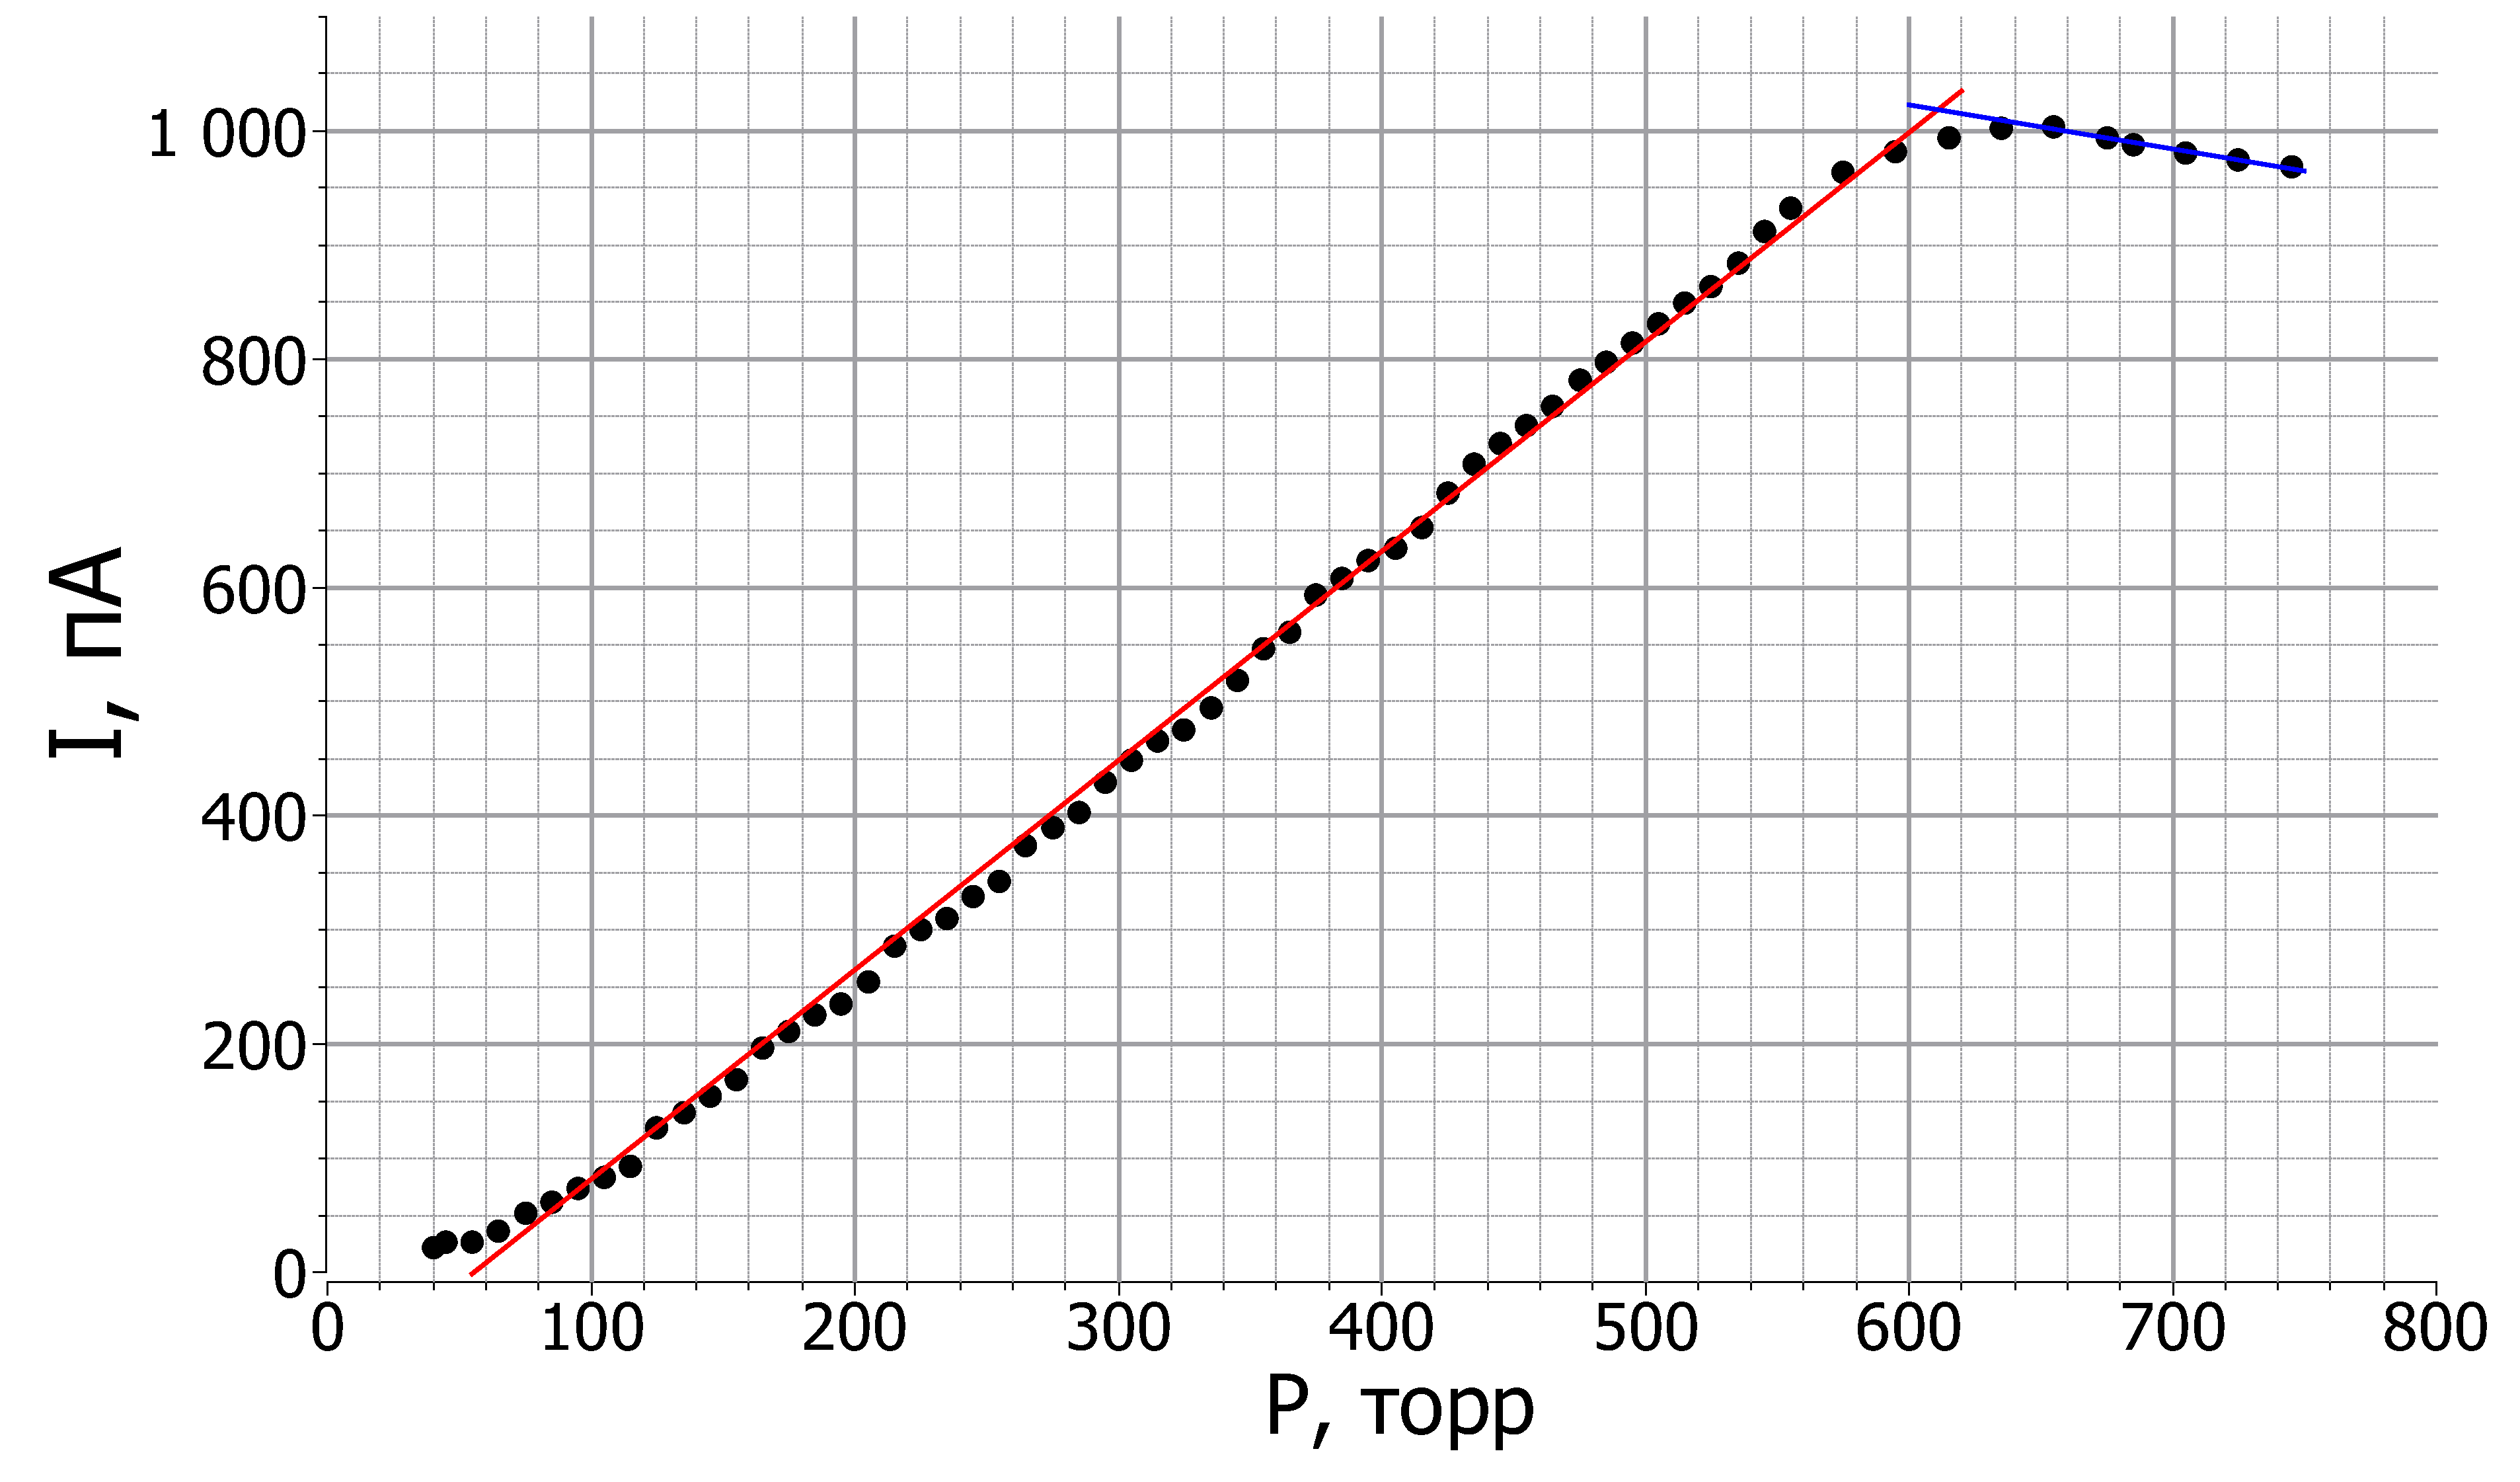
\includegraphics[width=\linewidth]{Pictures/Ionization_Plot.pdf}
			\caption{Зависимость $I(P)$}
		\end{figure}
	
		Посчитаем энергию $\alpha$-частиц:
		\begin{equation*}
			\boxed{E = (5,22 \pm 0,05) \text{ МэВ}}
		\end{equation*}
	
		В этот раз значение чрезвычайно близко к истинному $E = 5,15$ МэВ! 
	
	\end{enumerate}

	\newpage
	\tocsection{Вывод}
	
	\begin{table}[h!]
		\centering
		\resizebox{\columnwidth}{!}{%
			\begin{tabular}{c|c|c|c|}
				\cline{2-4}
				& Счетчик Гейгера & Сцинтилляционный счетчик & Ионизационная камера \\ \hline
				\multicolumn{1}{|c|}{$R_\text{э}$, см}                   & $1,9 \pm 0,3$   & $2,4 \pm 0,2$            & $3,82 \pm 0,06$      \\ \hline
				\multicolumn{1}{|c|}{$R_\text{ср}$, см}                  & $1,77 \pm 0,05$ & $1,32 \pm 0,05$          & --                   \\ \hline
				\multicolumn{1}{|c|}{$R'_\text{э}$, $10^{-3}$ г/см$^2$}  & $2,2 \pm 0,4$   & $2,8 \pm 0,2$            & $4,47 \pm 0,07$      \\ \hline
				\multicolumn{1}{|c|}{$R'_\text{ср}$, $10^{-3}$ г/см$^2$} & $2,07 \pm 0,06$ & $1,55 \pm 0,06$          & --                   \\ \hline
				\multicolumn{1}{|c|}{$E_\text{э}$, МэВ}                  & $3,3 \pm 0,4$   & $3,8 \pm 0,2$            & $5,22 \pm 0,05$      \\ \hline
				\multicolumn{1}{|c|}{$E_\text{ср}$, МэВ}                 & $3,13 \pm 0,06$ & $2,9 \pm 0,1$            & --                   \\ \hline
			\end{tabular}%
		}
	\end{table}
	
	В данной работе мы измерили пробег $\alpha$-частиц в воздухе. Получили достаточно много разных значений, неслабо отличающихся друг от друга. Однако они все оказываются одного порядка и даже того же порядка, что и истинное значение. Это же верно и для найденных энергий $\alpha$-частиц. Значения, найденные с помощью счетчика Гейгера и сцинтилляционного счетчика, занижены по сравнению с реальным значением. Лучше всего к действительности подобрался способ с ионизационной камерой: $E = (5,22 \pm 0,05)$ МэВ; в то время как настоящее значение $E = 5,15$ МэВ. Заниженные значения в первых двух методах объясняется несовершенством методики: $\alpha$-частицы тратят свою энергию на преодоление дополнительных препятствий. 
	
	
	
\end{document}